\documentclass[a4paper, fontsize=14pt]{article}
\usepackage{scrextend}
\usepackage{indentfirst, fancyhdr, amsfonts, mathtools, amssymb}
\usepackage{titlesec} %работа с рубрикацией
\usepackage{tocloft} %настройки оглавления
\usepackage[T2A]{fontenc}
\usepackage[utf8x]{inputenc}
\usepackage[russian]{babel}
\usepackage{hyperref} %кликабельное оглавление
\usepackage[left=3.7cm,right=2cm,top=2cm,bottom=2cm]{geometry}
\usepackage{tempora} %настраиваем шрифт типа TNR                                   
\usepackage{newtxmath} %делаем шрифт формул похожим на TNR
\usepackage{caption}
\usepackage{listings}
\lstset{
  columns=fullflexible,
  breaklines=true,
}
\linespread{1}
\setcounter{page}{4} %в зависимости от того, какой по счёту страницей должно быть оглавление!

%НАСТРОЙКИ ОГЛАВЛЕНИЯ
\renewcommand{\cftsecaftersnum}{.} %точки после номеров разделов и подразделов в оглавлении
\renewcommand{\cftsubsecaftersnum}{.}
\renewcommand{\cftsecfont}{\normalfont} %разделы в оглавлении пишутся обычным (не жирным) шрифтом
\renewcommand{\cftsecpagefont}{\normalfont} %соответствующие им страницы тоже
\renewcommand{\cftsecleader}{\cftdotfill{\cftdotsep}} %расставляем точки между названиями разделов и их страницами
\addto\captionsrussian{\renewcommand\contentsname{СОДЕРЖАНИЕ}} %хотим, чтобы слово "Содержание" писалось капсом
\renewcommand{\cfttoctitlefont}{\hfil\bfseries} %слово СОДЕРЖАНИЕ по центру жирным
\renewcommand{\cftaftertoctitle}{\hfill}

%НАСТРОЙКИ РУБРИКАЦИИ
\titleformat*{\section}{\center\bf} %названия разделов и подразделов по середине жирным шрифтом
\titleformat*{\subsection}{\center\bf}
\titlelabel{\thetitle.\quad} %название раздела и его номер отделены точкой

%НАСТРОЙКИ БИБЛИОГРАФИИ
\addto\captionsrussian{\renewcommand\refname{СПИСОК ЛИТЕРАТУРЫ}} %хотим, чтобы слова "Список литературы" писались капсом
\makeatletter
\renewcommand{\@biblabel}[1]{#1.} %хотим, чтобы в списке литературы номера источников писались в формате "No. <...>", а не "[No] <...>"
\makeatother

\begin{document}
\textbf{Цель работы:} получить навык численного решения нелинейных уравнений и систем таких уравнений.
\subsection*{{Ход работы}}

Необходимо найти значения корней с погрешностью $\varepsilon = 10^{-6}$ на отрезке $x\in[4,6]$ функции: 
\begin{equation}
    \label{eq:target_func}
    2 \sin(x^2) - 1 = 0
\end{equation}

\begin{center}
    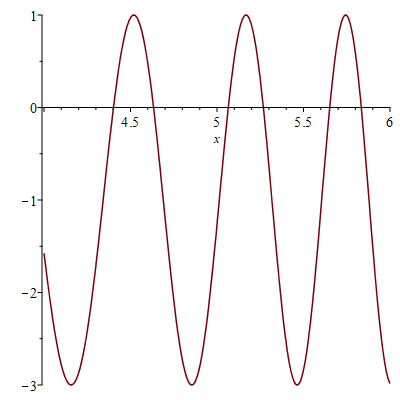
\includegraphics[scale=0.6]{src/target_plot.png}
    \captionof{figure}{График функции $2 \sin(x^2) - 1 = 0$}
    \label{fig:target_plot}
\end{center}

График функции \eqref{eq:target_func} продемонстрирован на рисунке \ref{fig:adaptive_plot}. Видно, что функция имеет на нем 6 различных корней. 
Заметим, что уравнение \eqref{eq:target_func} можно решить явно аналитически, получив корни:
\begin{equation*}
    \begin{aligned}
        x = \pm \sqrt{\frac{\pi}{6} + 2 \pi n} \\
        x = \pm \sqrt{\frac{5 \pi}{6} + 2 \pi n}
    \end{aligned}
\end{equation*}

На отрезке $[4, 6]$ получим соответственно:
\begin{equation*}
    \begin{aligned}
        x_1 \approx 4.4014946\\
        x_2 \approx 4.6333087\\
        x_3 \approx 5.0652087\\
        x_4 \approx 5.2678966\\
        x_5 \approx 5.6515064\\
        x_6 \approx 5.8338598
    \end{aligned}
\end{equation*}
\subsubsection*{Задача №1}
\begin{enumerate}
\item Написать вычислительную программу на языке программирования C++ для решения нелинейного уравнения на указанном отрезке с заданной точностью методом:
\begin{itemize}
    \item бисекции (дихотомии) (1 балл),
    \item хорд (1 балл),
    \item простых итераций (1 балл),
    \item касательных (Ньютона) (1 балл),
    \item секущих (1 балл).
\end{itemize}
Программа должна предусматривать возможность нахождения всех
корней уравнения с заданной точностью.
\item С использованием написанной программы решить нелинейное уравнение
согласно индивидуальному заданию.
\item Выполнить сравнительный анализ реализованных методов
\end{enumerate}
\subsubsection*{Решение}

Построим метод простых итераций, домножим \eqref{eq:target_func} на $\alpha = 0.01$ и прибавим $x$ в обе части.
Получим итерационный процесс:
\begin{equation}
    x_{k+1} = x_{k} + 0.02 \sin(x^2_k) - 0.01 = \phi_{+}(x);
\end{equation}

\begin{center}
    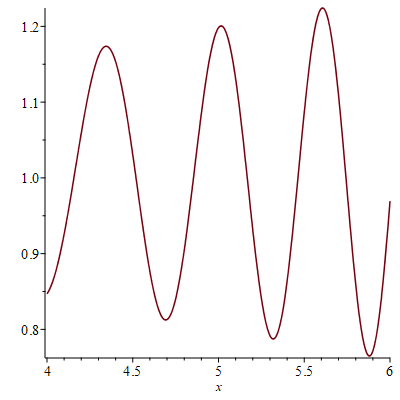
\includegraphics[scale=0.6]{src/simple_iter_pos.png}
    \captionof{figure}{График $\phi_{+}'(x) = 0.04 x \cos(x^2) + 1$ }
    \label{fig:simple_iter_pos}
\end{center}
График производной $\phi_{+}'(x)$ продемострирован на рисунке \ref{fig:simple_iter_pos}. Видно, что он принимает значения по модулю меньше, чем $1$ в окрестности точек $x_2, x_4, x_6$.

Аналогично можно построить итерационный процесс $\alpha = - 0.01$:
\begin{equation}
    x_{k+1} = x_{k} - 0.02 \sin(x^2_k) + 0.01 = \phi_{-}(x);
\end{equation}

\begin{center}
    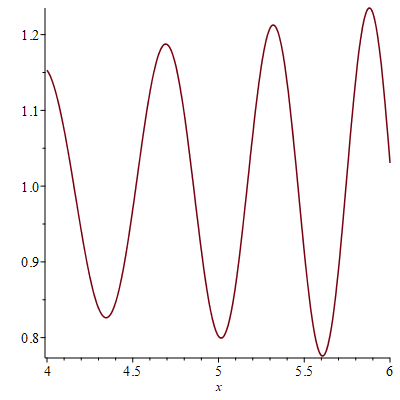
\includegraphics[scale=0.6]{src/simple_iter_neg.png}
    \captionof{figure}{График $\phi'_{-}(x) = -0.04 x \cos(x^2) + 1$ }
    \label{fig:simple_iter_neg}
\end{center}

График производной $\phi_{-}'(x)$ продемострирован на рисунке \ref{fig:simple_iter_neg}. Заметим, что $|\phi_{-}(x)|$ принимает значения меньше, чем $1$ в окрестности точек $x_1, x_3, x_5$.

Полученные итерационные процессы при достаточно близком задании к точкам $x_i$ сходятся к каждой из них.

Если же выбрать $\alpha(x) = - \frac{1}{f'(x)}$, то получим метод Ньютона:
\begin{equation}
    x_{k+1} = x_k - \frac{2 \sin(x^2) - 1}{4 x \cos(x^2)} = \phi(x)
\end{equation}

Тогда, 

\begin{equation}
    \label{eq:newton_phi_prime}
    |\phi'(x)| = \left| \frac{2 \sin(x^2) - 1}{4 x^2 \cos(x^2)} - \frac{(2 \sin(x^2) - 1) \sin(x^2)}{2 \cos^2(x^2)} \right|
\end{equation}

\begin{center}
    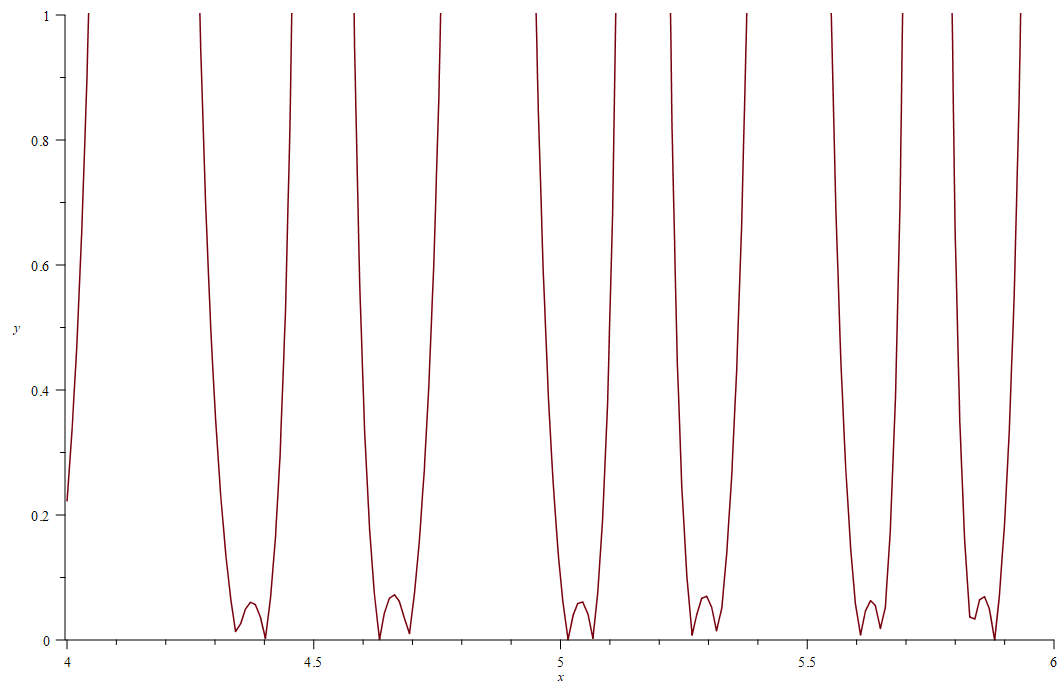
\includegraphics[scale=0.4]{src/newton_iter.png}
    \captionof{figure}{График функции \eqref{eq:newton_phi_prime}}
    \label{fig:newton_phi}
\end{center}


График модуля производной $\phi(x)$ продемонстирован на рисунке \ref{fig:newton_phi}. Только в окрестности точек $x_i$ значение $| phi'(x) |< 1$, 
таким образом, построенный итерационный процесс сходится к ним не с любой начальной точки.

Метод секущих получается из метода касательных заменой $f'(x_k)$ разностным приближением: 
\begin{equation*}
    f'(x_k) \approx \frac{f(x_k) - f(x_{k-1})}{x_k - x_{k-1}}
\end{equation*}

Таким образом,

\begin{equation*}
    x_{k+1} = x_k -  \frac{x_k - x_{k-1}}{f(x_k) - f(x_{k-1})} f(x^k)
\end{equation*}

Полученные результаты для методов из пункта 1 продемонстрированы на рисунке \ref{fig:result1} для уравнения \eqref{eq:target_func}.
Методы, основанные на методе простых итераций оказались хуже в виду того, что при выделении корня $x = \phi(x)$, производная $| \phi(x) | $ сильно осциллирует.


\begin{center}
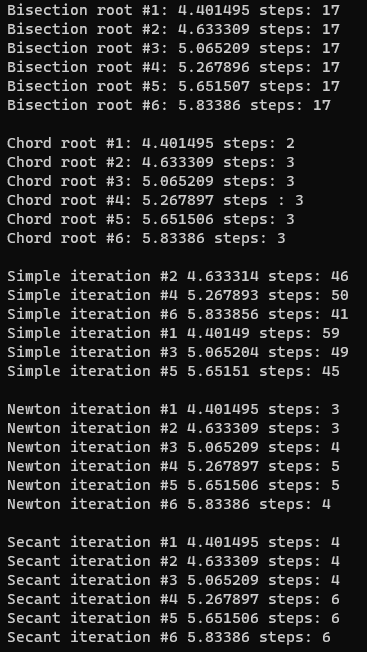
\includegraphics{src/result_1.png}
    \captionof{figure}{Результат работы программы для Задания 1}
    \label{fig:result1}
\end{center}

\subsubsection*{Задача №2}
\begin{enumerate}
    \item Написать вычислительную программу на языке программирования C++ для решения системы двух нелинейных уравнений методом простых итераций с заданной точностью.
    \item С использованием написанной программы найти численно минимум
    заданной функции двух переменных $F(x,y)$ в указанной области путем
    численного решения системы двух нелинейных уравнений, получающихся
    на основе необходимых условий экстремума.
\end{enumerate}
\subsubsection*{Решение}

Дана функция:
\begin{equation}
    \label{eq:simpleiterminmax_target}
    F(x,y) = x^2 + y^2 + (x+y+1) \operatorname{tg} (x+y), \quad [-0.5, 0] \times [-0.5, 0]
\end{equation}

График функции продемонстрирован на рисунке \ref{fig:simpleiterminmax_target_plot}.

\begin{center}
    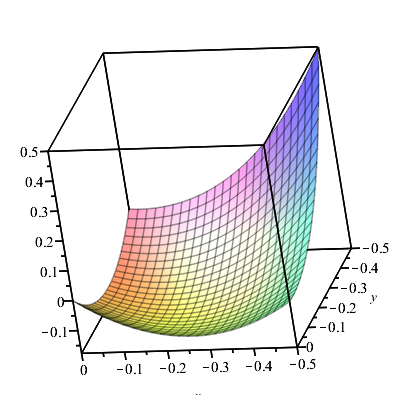
\includegraphics[scale=0.5]{src/simple iter sys target.png}
    \captionof{figure}{График функции $F(x, y), x \in [-0.5, 0], y \in [-0.5, 0]$}
    \label{fig:simpleiterminmax_target_plot}
\end{center}

Условие экстремума:
\begin{equation}
    \label{eq:exstr_condition}
    \begin{aligned}
        F_x =  2 x + \operatorname{tg}(x+y) + (x+y+1) (1 + \operatorname{tg}^2 (x+y)) = 0 \\
        F_y =  2 y + \operatorname{tg}(x+y) + (x+y+1) (1 + \operatorname{tg}^2 (x+y)) = 0\\
    \end{aligned}
\end{equation}


Получили систему нелиненых уравнений. Умножим первое уравнение системы \eqref{eq:exstr_condition} на  $-0.0001$ и прибавим $x$ в обе части.
Второе уравнение также умножим на на  $-0.0001$ и прибавим $y$ в обе части. Получим итерационный процесс, причем в окрестности $(-0.176, -0.176)$ выполнено:
\begin{equation*}
    \begin{aligned}
        &\left| \frac{\partial F_x(x)}{\partial x}  \right| +  \left| \frac{\partial F_x(x)}{\partial y} \right| < 1 \\
        &\left| \frac{\partial F_y(x)}{\partial x}  \right| +  \left| \frac{\partial F_y(x)}{\partial y} \right| < 1
    \end{aligned}
\end{equation*}
причем в самой точке значение левой части равно $0.998$. 

Результат работы программы с данным итерационным процессом продемонстрирован на рисунке \ref{fig:simpleiterminimum}.

\begin{center}
    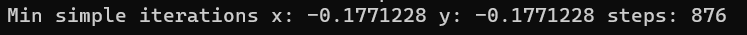
\includegraphics[scale=0.8]{src/simple iter minimum.png}
    \captionof{figure}{Результат работы программы для задания 2}
    \label{fig:simpleiterminimum}
\end{center}

Процесс долго сходится и даёт результат с погрешностью $\varepsilon = 0.001$ от эталонного решения в пакете Maple ($\overline{x} = -0.1789519, \overline{y} = -0.1789519$).

\subsubsection*{Задача №3}
\begin{enumerate}
    \item Написать вычислительную программу на языке программирования C++
    для решения системы двух нелинейных уравнений методом Ньютона. При
    этом предусмотреть две возможности: a) точное задание всех
    производных, б) приближенное вычисление производных по точно
    заданным функциям с заданной точностью.
    \item С использованием написанной программы решить задачу о поиске
    минимума функции двух переменных $F(x,y)$ сведением к системе двух
    нелинейных уравнений с использованием необходимого условия
    экстремума. Выполнить сравнительный анализ двух указанных в п.1)
    реализаций метода.
\end{enumerate}
\subsubsection*{Решение}

Результат работы программы методом Ньютона решения систем нелинейных уравнений продемонстрирован на рисунке \ref{fig:simpleiterminimum}.

\begin{center}
    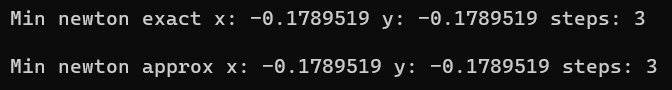
\includegraphics[scale=0.8]{src/newton minimum prog.png}
    \captionof{figure}{Результат работы программы для задания 3}
    \label{fig:simpleiterminimum}
\end{center}

Здесь exact - с заданием точных формул, approx - с их численной аппроксимацией.

Процесс сходится быстро и совпадает с эталонным решением в пакете Maple ($\overline{x} = -0.1789519, \overline{y} = -0.1789519$).

\newpage
\subsection*{Вывод}
В результате проделанной лабораторной работы был получен навык численного решения нелинейных уравнений и систем таких уравнений.
\newpage
\subsection*{Список литературы}
\begin{enumerate}
    \item Бахвалов Н.С., Жидков Н.П., Кобельков Г.М. Численные методы: Бином, 2018. – 636 с. 
    \item Калиткин Н.Н. Численные методы, 2-е издание: БХВ-Петербург, 2014. – 592 с.
    \item Самарский А.А., Гулин А. В. Численные методы: Учеб, пособие для вузов, — М.: Наука. Гл. ред. физ-мат. лит., 1989.— 432 с.
\end{enumerate}
\newpage
\subsection*{Приложение}
Весь код выложен в github-репозитории по ссылке: 

\url{https://github.com/sultanovMF/Numerical-Methods-Lab}

\end{document}


